%===============================================================================
% LaTeX sjabloon voor de bachelorproef toegepaste informatica aan HOGENT
% Meer info op https://github.com/HoGentTIN/latex-hogent-report
%===============================================================================

\documentclass[dutch,dit,thesis]{hogentreport}

% TODO:
% - If necessary, replace the option `dit`' with your own department!
%   Valid entries are dbo, dbt, dgz, dit, dlo, dog, dsa, soa
% - If you write your thesis in English (remark: only possible after getting
%   explicit approval!), remove the option "dutch," or replace with "english".

\usepackage{lipsum} % For blind text, can be removed after adding actual content

%% Pictures to include in the text can be put in the graphics/ folder
\graphicspath{{graphics/}}

%% For source code highlighting, requires pygments to be installed
%% Compile with the -shell-escape flag!
\usepackage[section]{minted}
\usemintedstyle{solarized-light}
\definecolor{bg}{RGB}{253,246,227} %% Set the background color of the codeframe

%% Change this line to edit the line numbering style:
\renewcommand{\theFancyVerbLine}{\ttfamily\scriptsize\arabic{FancyVerbLine}}

%% Macro definition to load external java source files with \javacode{filename}:
\newmintedfile[javacode]{java}{
    bgcolor=bg,
    fontfamily=tt,
    linenos=true,
    numberblanklines=true,
    numbersep=5pt,
    gobble=0,
    framesep=2mm,
    funcnamehighlighting=true,
    tabsize=4,
    obeytabs=false,
    breaklines=true,
    mathescape=false
    samepage=false,
    showspaces=false,
    showtabs =false,
    texcl=false,
}

% Other packages not already included can be imported here

%%---------- Document metadata -------------------------------------------------
% TODO: Replace this with your own information
\author{Maarten Eylenbosch}
\supervisor{Dhr. L. Smits}
\cosupervisor{Mnr. R. Timmermans}
\title[Optionele ondertitel]%
    {Maturiteit van IBM Db2 Administration Foundation for z/OS}
\academicyear{\advance\year by -1 \the\year--\advance\year by 1 \the\year}
\examperiod{1}
\degreesought{\IfLanguageName{dutch}{Professionele bachelor in de toegepaste informatica}{Bachelor of applied computer science}}
\partialthesis{false} %% To display 'in partial fulfilment'
%\institution{Internshipcompany BVBA.}

%% Add global exceptions to the hyphenation here
\hyphenation{back-slash}

%% The bibliography (style and settings are  found in hogentthesis.cls)
\addbibresource{bachproef.bib}            %% Bibliography file
\addbibresource{../voorstel/voorstel.bib} %% Bibliography research proposal
\defbibheading{bibempty}{}

%% Prevent empty pages for right-handed chapter starts in twoside mode
\renewcommand{\cleardoublepage}{\clearpage}

\renewcommand{\arraystretch}{1.2}

%% Content starts here.
\begin{document}

%---------- Front matter -------------------------------------------------------

\frontmatter

\hypersetup{pageanchor=false} %% Disable page numbering references
%% Render a Dutch outer title page if the main language is English
\IfLanguageName{english}{%
    %% If necessary, information can be changed here
    \degreesought{Professionele Bachelor toegepaste informatica}%
    \begin{otherlanguage}{dutch}%
       \maketitle%
    \end{otherlanguage}%
}{}

%% Generates title page content
\maketitle
\hypersetup{pageanchor=true}

\input{voorwoord}
\input{samenvatting}

%---------- Inhoud, lijst figuren, ... -----------------------------------------

\tableofcontents

% In a list of figures, the complete caption will be included. To prevent this,
% ALWAYS add a short description in the caption!
%
%  \caption[short description]{elaborate description}
%
% If you do, only the short description will be used in the list of figures

\listoffigures

% If you included tables and/or source code listings, uncomment the appropriate
% lines.
%\listoftables
%\listoflistings

% Als je een lijst van afkortingen of termen wil toevoegen, dan hoort die
% hier thuis. Gebruik bijvoorbeeld de ``glossaries'' package.
% https://www.overleaf.com/learn/latex/Glossaries

%---------- Kern ---------------------------------------------------------------

\mainmatter{}

% De eerste hoofdstukken van een bachelorproef zijn meestal een inleiding op
% het onderwerp, literatuurstudie en verantwoording methodologie.
% Aarzel niet om een meer beschrijvende titel aan deze hoofdstukken te geven of
% om bijvoorbeeld de inleiding en/of stand van zaken over meerdere hoofdstukken
% te verspreiden!

\input{inleiding}
\input{standvanzaken}
\input{methodologie}

% Voeg hier je eigen hoofdstukken toe die de ``corpus'' van je bachelorproef
% vormen. De structuur en titels hangen af van je eigen onderzoek. Je kan bv.
% elke fase in je onderzoek in een apart hoofdstuk bespreken.

%\input{...}
%\input{...}
%...

\input{conclusie}

%---------- Bijlagen -----------------------------------------------------------

\appendix

\chapter{Onderzoeksvoorstel}

Het onderwerp van deze bachelorproef is gebaseerd op een onderzoeksvoorstel dat vooraf werd beoordeeld door de promotor. Dat voorstel is opgenomen in deze bijlage.

%% TODO: 
%\section*{Samenvatting}

Dit onderzoek bekijkt of IBM Db2 Administration Foundation matuur genoeg is om IBM Db2 Data Studio te vervangen binnenin een productieomgeving op Mainframe. Dit gebeurt aan de hand van een vergelijkende studie tussen een Proof of Concept van de nieuwe configuratie en de huidige configuratie. 

% Verwijzing naar het bestand met de inhoud van het onderzoeksvoorstel
%---------- Inleiding ---------------------------------------------------------

\section{Introductie}%
\label{sec:introductie}

Het database management systeem dat KBC voor z/OS gebruikt is Db2. Voor het beheer hiervan maken ze gebruik van IBM Data Studio. Deze software krijgt echter geen nieuwe features meer en willen ze binnen enkele jaren vervangen.

IBM Db2 Administration Foundation for z/OS, de nieuwe Db2 administratie software van IBM moet eerst voldoende ontwikkeld zijn voor KBC ze deze wilt binnenhalen. Dit onderzoek zal aan de hand van een Proof of Concept deze software beoordelen.

Op de testomgeving van KBC zullen Db2 Administration Foundation en andere benodigde software eerst geïnstalleerd en geconfigureerd worden. Daarna volgt een onderzoek van deze configuratie naar onder andere maturiteit, veiligheid, functionaliteit, enz. 

Dit onderzoek zal afhankelijk van deze ondervindingen in vergelijking met de huidige installatie bestuderen of deze software Data Studio reeds kan vervangen en of het voor KBC interessant is om deze nieuwe IBM software aan te schaffen.


%---------- Stand van zaken ---------------------------------------------------

\section{State-of-the-art}%
\label{sec:state-of-the-art}

Een mainframe is een computer die gebruikt wordt voor kritieke toepassingen vanwege hoge performantie, stabiliteit en veiligheid \autocite{IBM}. Dankzij de capaciteit om duizenden transacties per seconde te verwerken staat het mainframe centraal in de infrastructuur van bedrijven zoals KBC \autocite{IBM2010}.

Het voornaamste besturingssysteem voor mainframes is IBM z/OS. Dit is een 64-bit besturingssysteem dat als grote kracht heeft dat het achterwaarts compatibel is. Daarnaast kan bijvoorbeeld Linux of Windows ook op mainframes draaien \autocite{MaryE.Shacklett2022}.

De omgeving die in dit onderzoek bekeken wordt, maakt gebruikt van Logical Partitions (LPARs), dit zijn partities in een z/OS systeem die zich als onafhankelijke systemen kunnen gedragen \autocite{IBM2010a}.

De testomgeving voor onze proof of concept zit op een aparte LPAR afgeschermd van de productieomgeving.
Db2 for z/OS is een relationeel database management systeem \autocite{IBM2022a}.

KBC gebruikt momenteel voor het beheer van zijn Db2 instanties IBM Data Studio. Deze tool is gebaseerd op Eclipse en heeft veel van dezelfde functionaliteiten zoals bijvoorbeeld plugins \autocite{IBM2021}.

De verbinding tussen Data Studio en Db2 gebeurt dankzij Db2 Connect \autocite{IBM2022b}. Men gebruikt ook een IBM Db2 Analytics Accelerator (IDAA) voor grote en dure Db2 query’s. Dit is een bijkomende hardware en software dat via ethernet in verbinding staat met het mainframe \autocite{Bruni2012}. 

IBM Db2 Administration Foundation for z/OS (ADF) is een software voor het beheer van Db2. Deze software maakt deel uit van de IBM Unified Management Server for z/OS (UMS). Dit software pakket wordt gebruikt via IBM Unified Experience for z/OS, een grafische interface die draait op Zowe \autocite{IBM2022c}.

\begin{figure}[h]
    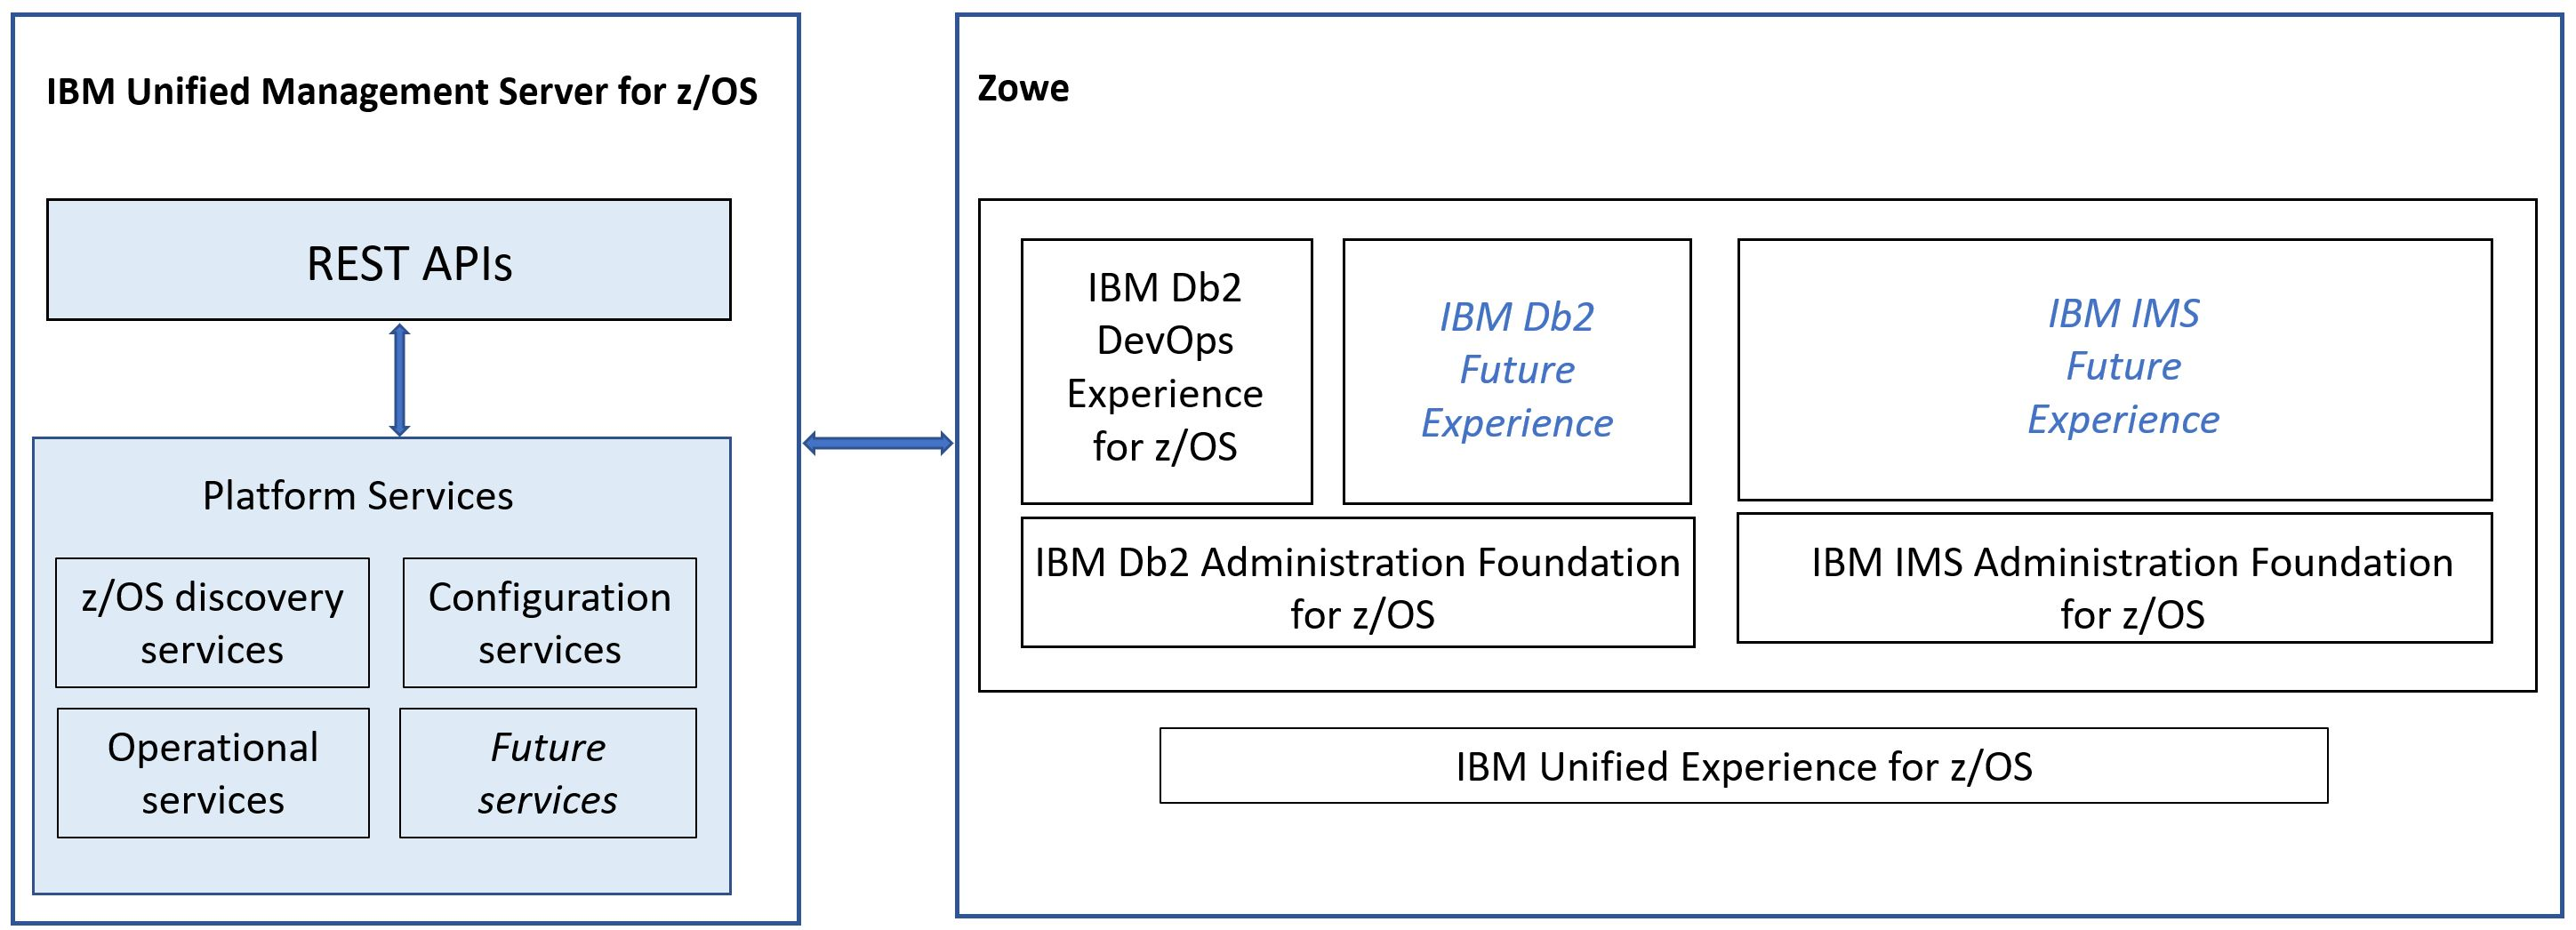
\includegraphics[scale=0.16]{UMS-ZOWE-ADF opstelling}
    \caption{Voorstelling van een configuratie met ADF \autocite{IBM2022c}}
\end{figure}

Zowe is een open source framework van het Open Mainframe Project, het zorgt voor moderne interfaces en manieren om met z/OS te werken via de browser. Het bevat ook een API mediation layer dat dient als toegangspunt voor REST APIs. Zowe bestaat uit onder andere een virtuele desktop, een command-line interface, een Visual Studio Code extension, enz \autocite{Zowe2022}.

REST staat voor representational state transfer, APIs worden gebruikt om informatie van programma’s of systemen op te halen. REST APIs sturen een voorstelling van de staat van de bron \autocite{RedHat2020}.

Om beheer van IDAA via ADF mogelijk te maken is ook de IBM DB2 Analysis Accelerator Administration Services software nodig. Deze software bestaat uit een aantal REST APIs en de user interface draait op Zowe \autocite{IBM2022d}.


%---------- Methodologie ------------------------------------------------------
\section{Methodologie}%
\label{sec:methodologie}

Dit onderzoek zal in eerste instantie bestaan uit een proof of concept. Op de testomgeving van KBC zullen Zowe, UMS,  IBM DB2 Analysis Accelerator Administration Services en ten slotte ADF geïnstalleerd en geconfigureerd worden.

Daarna zal men in de 2de fase van het onderzoek kijken of deze configuratie Data Studio bij KBC kan vervangen. Daarvoor volgt een vergelijkende studie tussen ADF en Data Studio op het vlak van onder andere de functionaliteiten van beide programma’s.

Ten slotte zal Administration Foundation zo uitgebreid mogelijk bekritiseerd worden naar enkele aanvullende eisen van KBC. Deze bijkomende criteria zijn de mogelijkheid tot Multi Factor Authenticatie, de levensduur van de verschillende programma’s in de configuratie en de frequentie van onderhoud en updates en hoeveel resources deze configuratie gebruikt op de testomgeving en welke impact zou dit hebben op de productieomgeving.



%---------- Verwachte resultaten ----------------------------------------------
\section{Verwacht resultaat, conclusie}%
\label{sec:verwachte_resultaten}

Het verwachte resultaat zal een combinatie zijn van de Proof of Concept en de studie naar de mogelijkheden van ADF in vergelijking met Data Studio. 

Hieruit zal zowel duidelijk zijn welke functionaliteiten reeds aanwezig zijn, de mogelijkheden die in Data Studio zitten en in ADF nog ontbreken en zaken die niet in Data Studio zitten maar wel in ADF.

Uit dit onderzoek zal ook blijken in hoeverre MFA mogelijk is en of ADF al stabiel genoeg is voor een productieomgeving op mainframe.

De verwachte conclusie is dat ADF een volwaardige vervanger voor Data Studio is en dat KBC klaar is om de overstap naar de nieuwe software te zetten.



%%---------- Andere bijlagen --------------------------------------------------
% TODO: Voeg hier eventuele andere bijlagen toe. Bv. als je deze BP voor de
% tweede keer indient, een overzicht van de verbeteringen t.o.v. het origineel.
%\input{...}

%%---------- Backmatter, referentielijst ---------------------------------------

\backmatter{}

\setlength\bibitemsep{2pt} %% Add Some space between the bibliograpy entries
\printbibliography[heading=bibintoc]

\end{document}
